% https://medium.com/xailient/face-detection-with-7-lines-of-code-in-python-5bf4cced34ac


\chapter{Face Detection with 7 Lines of Code in Python}

Only a few years ago, if someone asked me to work on a project that required detecting a person’s face using camera, to be honest, I would have shut down my laptop and run as far away from that person as possible because, first I knew that face detection was possible but not accessible to implement without domain knowledge and second, even if, somehow, I was able to make it work, it would probably take me a couple of months just to create a program that could detect faces.

It is a great time for us developers now, with tons of resources, libraries and how-to guides available, teaching and providing a much simpler way for us, without in-depth domain knowledge, to implement face detection.

In this post, I will show you how to create your own face detection program using Python with 7 lines of code.

You will need install the following if not already installed:

Python 3.7.3: For more information on downloading and installing refer to this \HREF{https://www.python.org/downloads/}{link}.

OpenCV: Install OpenCV if it is not already installed. You can either use apt install or pip3 install OpenCV.

\medskip

\SHELL{sudo apt install -y python3-opencv}

\medskip

or

\medskip

\SHELL{pip3 install opencv-python}

\medskip

tflite for Python 3.7: Please refer to \HREF{https://www.tensorflow.org/lite/guide/python}{guide} to this download the appropriate Python wheel for your system, and then install it with the pip3 installcommand.

Xailient FaceSDK: Please follow the instruction on this link to install the Xailient FaceSDK.


Here is the code to import the required python libraries, read an image from storage, perform face detection on the image and save the image with a bounding box around the detected faces in the same directory.

\begin{lstlisting}
import dnn
import cv2 as cv

im = cv.imread('image.jpg')
_, bboxes = dnn.FaceDetector().process_frame(im, threshold=0.4) 

for i in bboxes:    
    cv.rectangle(im, (i[0], i[1]), (i[2], i[3]), (0, 255, 0), 3)

cv.imwrite('/image_output.jpg', im)
\end{lstlisting}


Below are a few results of face detection using the above code.


You have your face detection program ready.

Found this post helpful? Leave your thoughts as comments below.

Originally published in \URL{www.xailient.com/blog}.

\section{How to Set Up Real-Time Face Detection on Raspberry Pi}

\subsection{A step-by-step guide to implement real-time face detection on a Raspberry Pi running 24 frames per second.}


In this post, I will guide you through a step-by-step process of implementing real-time face detection on a Raspberry Pi, running 24 frames per second on a single core.
    
For face detection, I will use Xailient FaceSDK.
    
\subsection{Set Up Your Raspberry Pi for Real-Time Face Detection}

\subsection{Step 1: Install Python 3.7.3}

Raspbian Buster comes with Python 3.7.3 preinstalled, so there is no need to explicitly install Python 3.7.3. To confirm, use the following command to see what version of Python is installed in your Raspberry Pi.

\medskip

\SHELL{python --version}    
    
\subsection{Step 2: Install tflite for Python 3.7}

To install tflite for Python 3.7, enter the following pip3 install command in your terminal.
    
\SHELL{pip3 install https:\\dl.google.com/coral/python/tflite\_runtime-1.14.0-cp37-cp37m-linuxarmv7l.whl}    

\subsection{Step 3: Install OpenCV}

    Install OpenCV if it is not already installed. You can either use apt install or pip3 install OpenCV on your Raspberry Pi.
    
    \SHELL{sudo apt install -y python3-opencv}
    
    or
    
    \SHELL{pip3 install opencv-python}
    
    
    
\subsection{Step 4: Download Xailient FaceSDK and Unzip}

    Go to Xailient SDK page and register as a new user and log in.
    
    Go to the SDK tab, where you will find instructions for downloading and installing Face SDK.
    
    
    For Raspberry Pi 3B+, download the ARM32 version of the SDK. You can either open the link from your Raspberry Pi’s browser to download it directly to it or you can use the following wget command:
    
\SHELL{wget -O sdk.tar.gz "SDKLINK"}


    
    Unzip the downloaded FaceSDK.
    
\subsection{Step 5: Add Shared Library to Path}


This is required as the library depends on some dynamically loaded shared Libraries.
    
\SHELL{export LD\_LIBRARY\_PATH=\$LD\_LIBRARY\_PATH:\$<Python\_SDK path/Shared\_arm32>}


    
    You can add a library path to bashrc script so that you don’t need to export every time you log in.

\SHELL{echo "export}    

\SHELL{LD\_LIBRARY\_PATH=\$LD\_LIBRARY\_PATH:\$<Python\_SDK path/Shared\_arm32" >> .bashrc}

    
\subsection{Step 6: Download Config File}

    From the Xailient SDK page, download the config file by either opening the link from your Raspberry Pi’s browser or using the following wget command:
    
    \SHELL{wget -O config.json "Config.Link"}

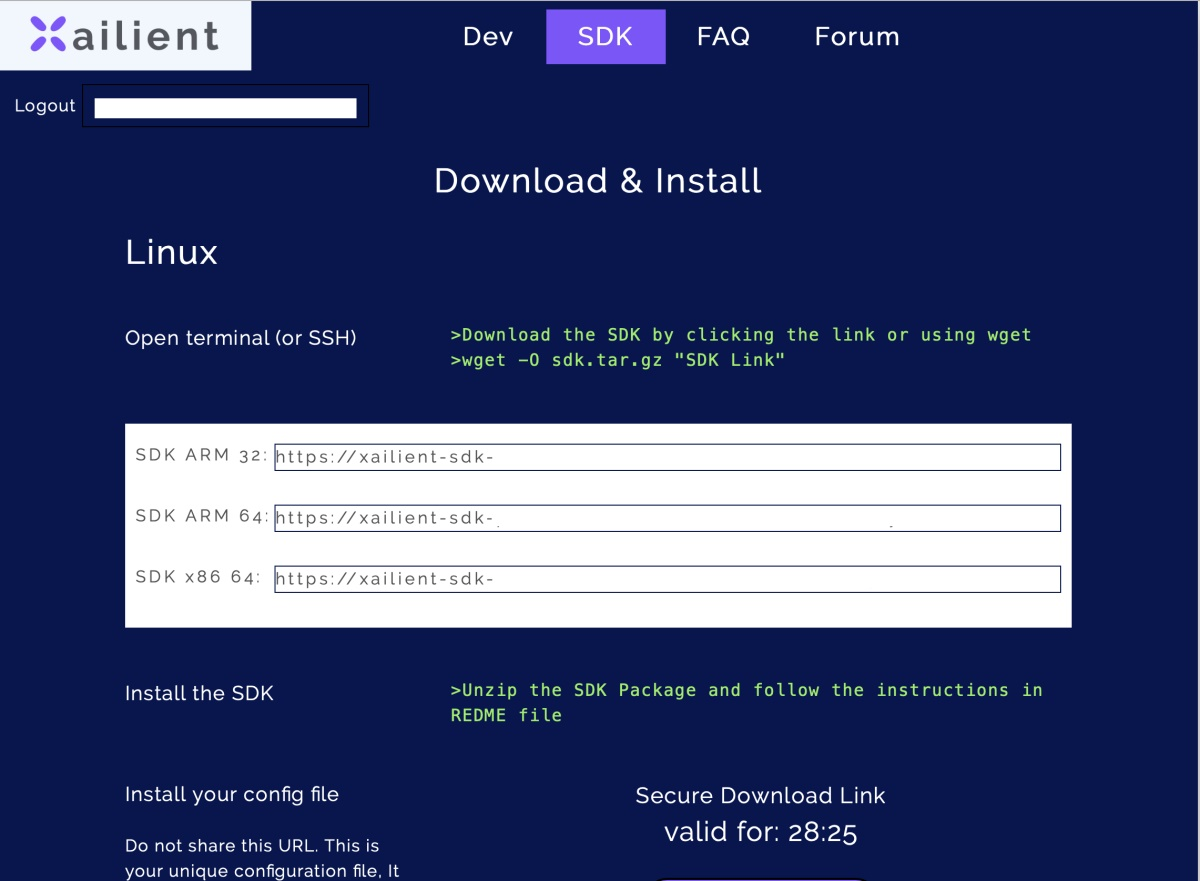
\includegraphics{Facedetection/RealTimeFaceDetectionOnARaspberryPi}    
    
    Copy the config.json file into the FaceSDK folder.

    
\subsection{Step 7: Install Xailient FaceSDK}

    To install the Xailient FaceSDK, run the file \FILE{Install.sh}  that is inside the SDK folder. Go to the FaceSDK folder from your terminal and run the following command: 
    
\SHELL{./Install.sh}    

    For more details on the installation process, you can refer to the Readme file that comes along with the FaceSDK.
    
\subsection{Step 8: Run Sample Face Detection Code}

    The FaceSDK comes with sample code that demonstrates how to use and interact with the Xailient Face Detector Python library.
    
    Go to the samples folder and run the \FILE{picam\_streaming\_demo.py} script to run real-time face detection.
    
    
    You now have real-time face detection running on a Raspberry Pi.
    
    Xailient is commercializing breakthrough university research in artificial intelligence and machine learning. Our technology dramatically reduces the costs of data transmission, storage, and computation associated with extracting useful information from real-time video by processing the way humans think.
    
    